\section{RANDCHI Generate Chi-Square Random Variable}

\subsection{Usage}

Generates a vector of chi-square random variables with the
given number of degrees of freedom.  The general syntax for
its use is 
\begin{verbatim}
   y = randchi(n)
\end{verbatim}
where \verb|n| is an array containing the degrees of freedom for
each generated random variable.
\subsection{Function Internals}

A chi-square random variable is essentially distributed as
the squared Euclidean norm of a vector of standard Gaussian random 
variables.  The number of degrees of freedom is generally the
number of elements in the vector.  In general, the PDF of
a chi-square random variable is
\[
 f(x) = \frac{x^{r/2-1}e^{-x/2}}{\Gamma(r/2)2^{r/2}}
\]
\subsection{Example}

First, a plot of the PDF for a family of chi-square random variables
\begin{verbatim}
--> f = zeros(7,100);
--> x = (1:100)/10;
--> for n=1:7;t=x.^(n/2-1).*exp(-x/2);f(n,:)=10*t/sum(t);end
--> plot(x,f');
\end{verbatim}
The PDF is below:


\centerline{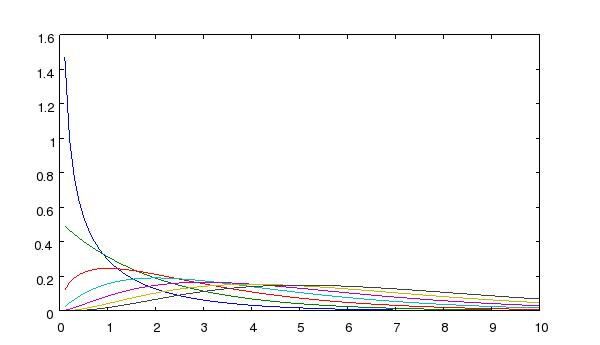
\includegraphics[width=8cm]{chipdf}}

Here is an example of using \verb|randchi| and \verb|randn| to compute
some chi-square random variables with four degrees of freedom.
\begin{verbatim}
--> randchi(4*ones(1,6))

ans = 
    2.6122    6.2362    0.8717    1.4935    6.0370    5.2771 

--> sum(randn(4,6).^2)

ans = 
    0.0399    4.6296    0.8697    0.5796    1.5490    5.8538 
\end{verbatim}
